\begin{figure}[!t]
	\centering
	\subfigure[CDF of layer sizes]{\label{fig_layer_size_cdf}
		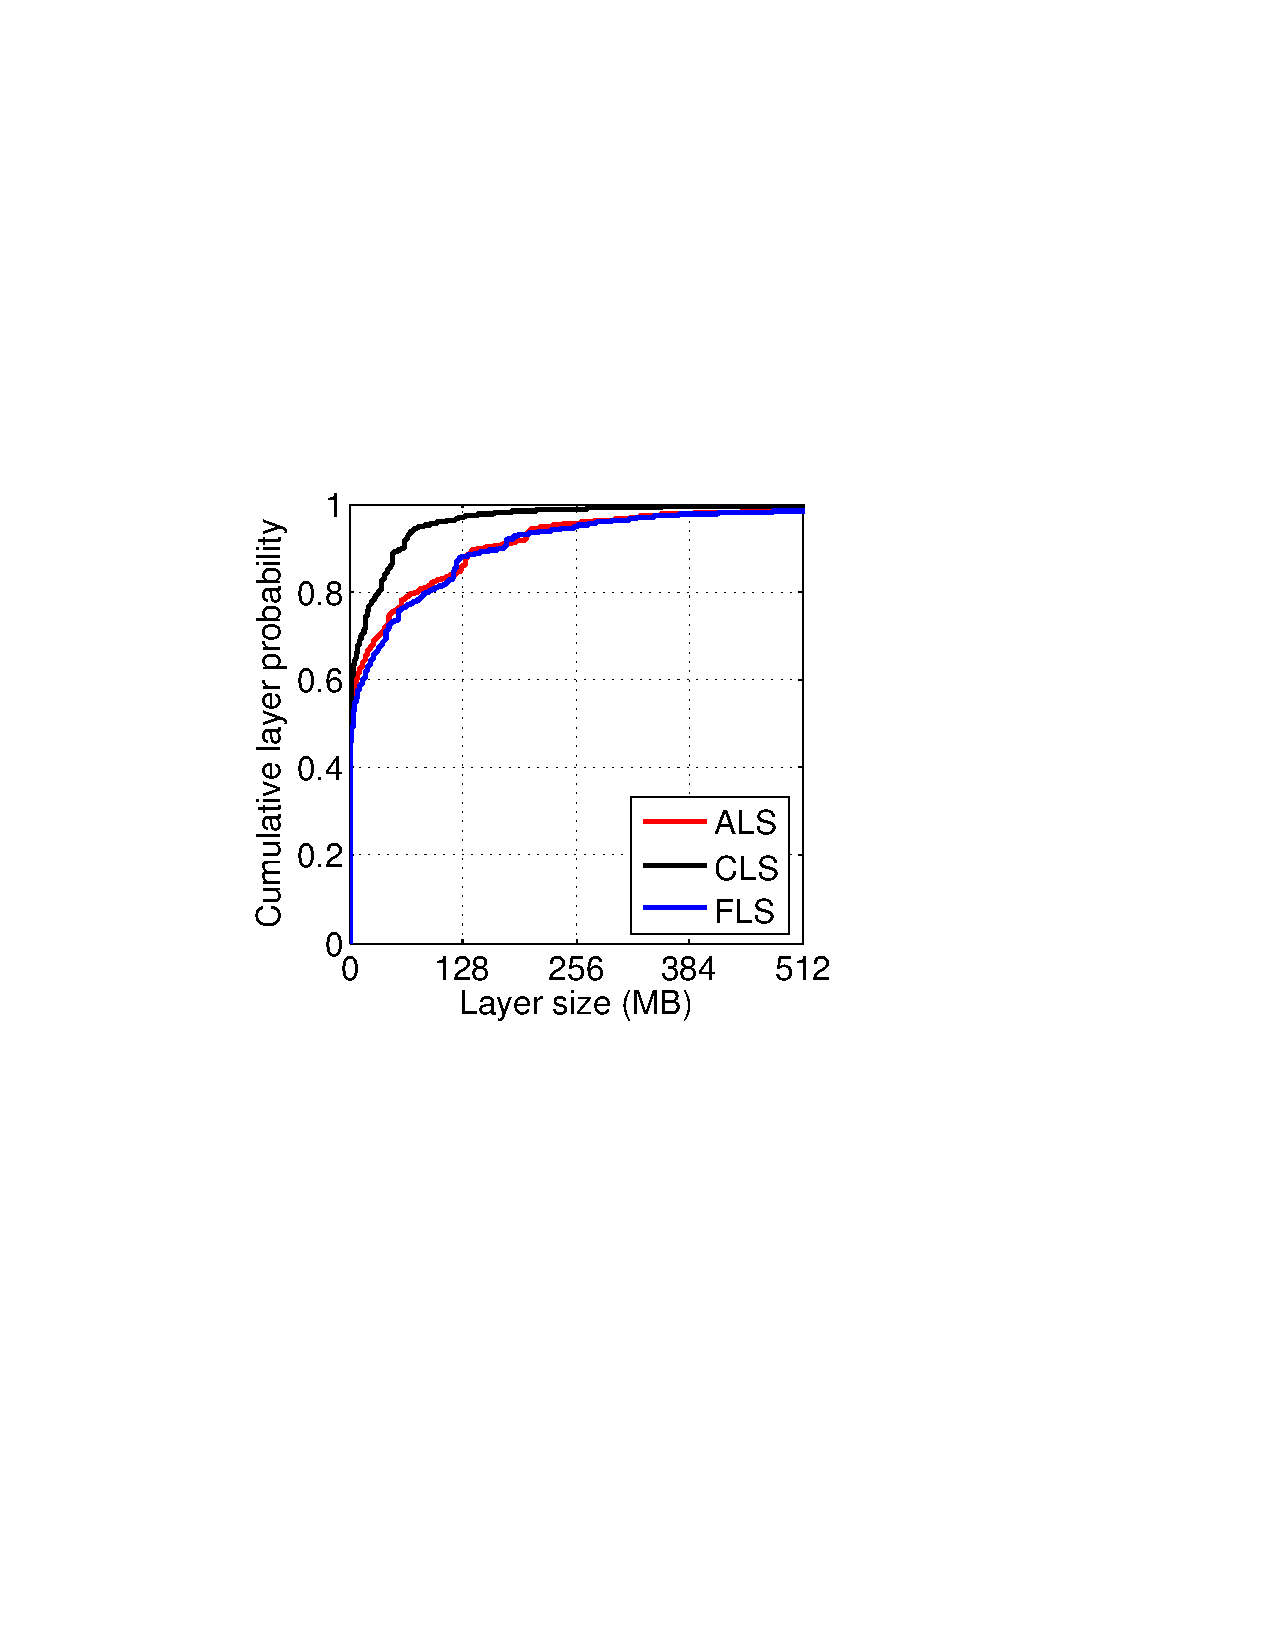
\includegraphics[width=0.23\textwidth]{graphs/layer_size_mb.pdf}
	}
	\subfigure[Histogram of layer sizes]{\label{fig_hist_layer_size}
		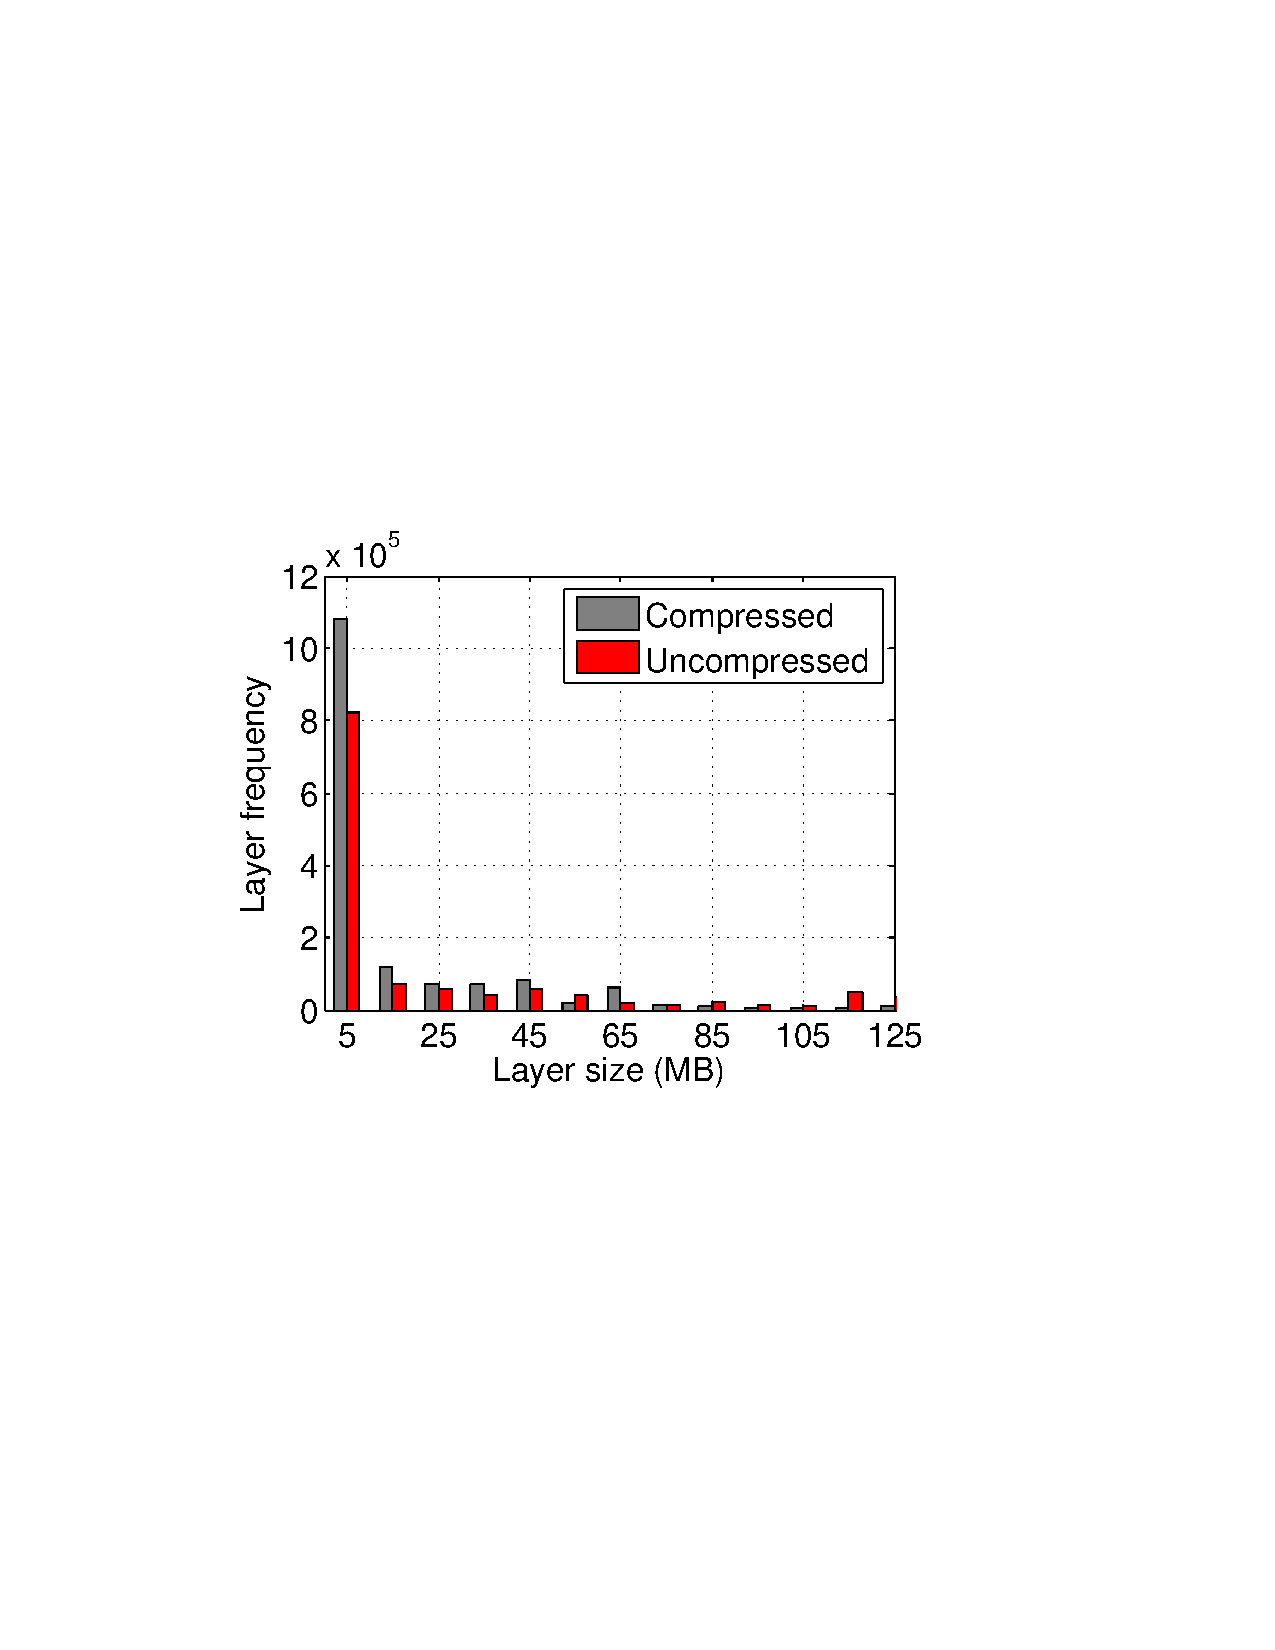
\includegraphics[width=0.223\textwidth]{graphs/hist_layer_size.pdf}
	}
	\caption{Layer size distribution
	\vcomment{Let's use CLS, ALS, and FLS abreviations}.
	\vcomment{CLS size should go first}.
	\vcomment{We need to use different types of lines (solid, dotted, etc.)
		or markers (round, triangular)}.
	\vcomment{In figure B it is not clear to which bar group corresponds
		  to which layer size. I suggest to try to rotate the graph
		  by 90 grads to fit all layer size labels.}
	}
	\label{fig-layer-size}
\end{figure}
